\documentclass[10pt]{beamer}

%% Chinese support
%% \usepackage[adobefonts,nocap]{ctex}

%% Fonts
\usepackage{multicol}
\usepackage{mathabx}
\usepackage[scaled]{helvet}
\usepackage{lmodern}
\usepackage{eulervm}
\usefonttheme[onlymath]{serif}
\usefonttheme{professionalfonts}
\usefonttheme{structurebold}
\usepackage{bm}
\usepackage{verbatim}

%% Color & Theme
\definecolor{SUblue}{RGB}{0,0,180}
\usecolortheme[RGB={0,0,180}]{structure}
\usetheme{Boadilla}
\setbeamertemplate{navigation symbols}{}
\setbeamertemplate{itemize items}[circle]
\setbeamertemplate{enumerate items}[circle]
\setbeamerfont{title}{size=\large}
\setbeamerfont{frametitle}{size=\large}
\setbeamerfont{framesubtitle}{size=\large,shape =$\color{violet}{\looparrowdownright}~$}
\setbeamercolor{title}{fg=white, bg= SUblue!75!green}
\setbeamercolor{framesubtitle}{fg=violet}
%\setlength{\leftmargini}{5pt}


\title[Statistical Computing]{{\textbf{Optimization}}}

\author[Feng Li]{\includegraphics[height=2cm]{cufelogo}\\
  \vspace{0.5cm}\textbf{Feng Li\\\texttt{feng.li@cufe.edu.cn}}}

\institute[SAM.CUFE.EDU.CN]{\footnotesize{\textbf{School of
      Statistics and Mathematics\\ Central University of Finance and
      Economics}}}
\date{}

%%%%%%%%%%%%%%%%%%%%%%%%%%%%%%%%%%%%%%%%%%%%%%%%%%%%%%%%%%%%%%%%%%%%%%
\begin{document}

%% Title page
\begin{frame}[plain]
  \titlepage
  \tiny{Revised on \today}
\end{frame}


%% Outline page
\section*{Today we are going to learn...}
\begin{frame}
  \frametitle{Today we are going to learn...}
  \tableofcontents
\end{frame}

\section{Newton-Raphson Algorithm}

\begin{frame}
  \frametitle{Newton-Raphson Algorithm}

  \begin{itemize}

  \item When the goal is to solve an equation of the form $f(x) = 0$,
      a common approach is to use a \textbf{Newton-Raphson algorithm},
      which produces a sequence such that


      \begin{equation*}
        x_{n+1} = x_n - \left( \frac{\partial f(x)}{\partial x}
          \mid_{x=x_n} \right)^{-1} f(x_n)
      \end{equation*}

    \item Note that $\frac{\partial f(x)}{\partial x}$ is the
      partial derivative for $f(x)$ with respect to $x$, also known
      as the \textbf{gradient}.

    \item $x$ can be a scaler or a vector.

  \end{itemize}

\end{frame}

\begin{frame}
  \frametitle{Example}

  \begin{itemize}
  \item Assume we want to find the root of $x^2 - b =0$ by using
    numerical method.

  \item First we have
    \begin{equation*}
      f'(x) = 2x
    \end{equation*}

  \item Then

    \begin{equation*}
        x_{n+1} = x_n - \left( 2x_n \right)^{-1} (x_n^2-b) = \frac{1}{2}(x_n+\frac{b}{x_n})
    \end{equation*}

  \end{itemize}

\end{frame}


\begin{frame}[fragile]
  \frametitle{The realization in R}
\begin{verbatim}
## The target function
f <- function(x, b) x^2 -b
## The gradient wrt x
df <- function(x, b) 2*x
## Loop to find the best x
n <- 50
x <- rep(NA, 1)
b <- 3
x[1] <- -100 # The initial value
for(i in 1:n)
{
    x[i+1] <- x[i]- (df(x[i], b))^(-1)*f(x[i], b)
}
## Check the convergence
par(mfrow = c(3, 1))
plot(x, type = "l", col = "red")
plot(f(x, b), type = "l", col = "red")
plot(df(x, b), type = "l", col = "red")
\end{verbatim}
\end{frame}

\begin{frame}
\frametitle{Diagnosis}

\begin{figure}
  \centering
  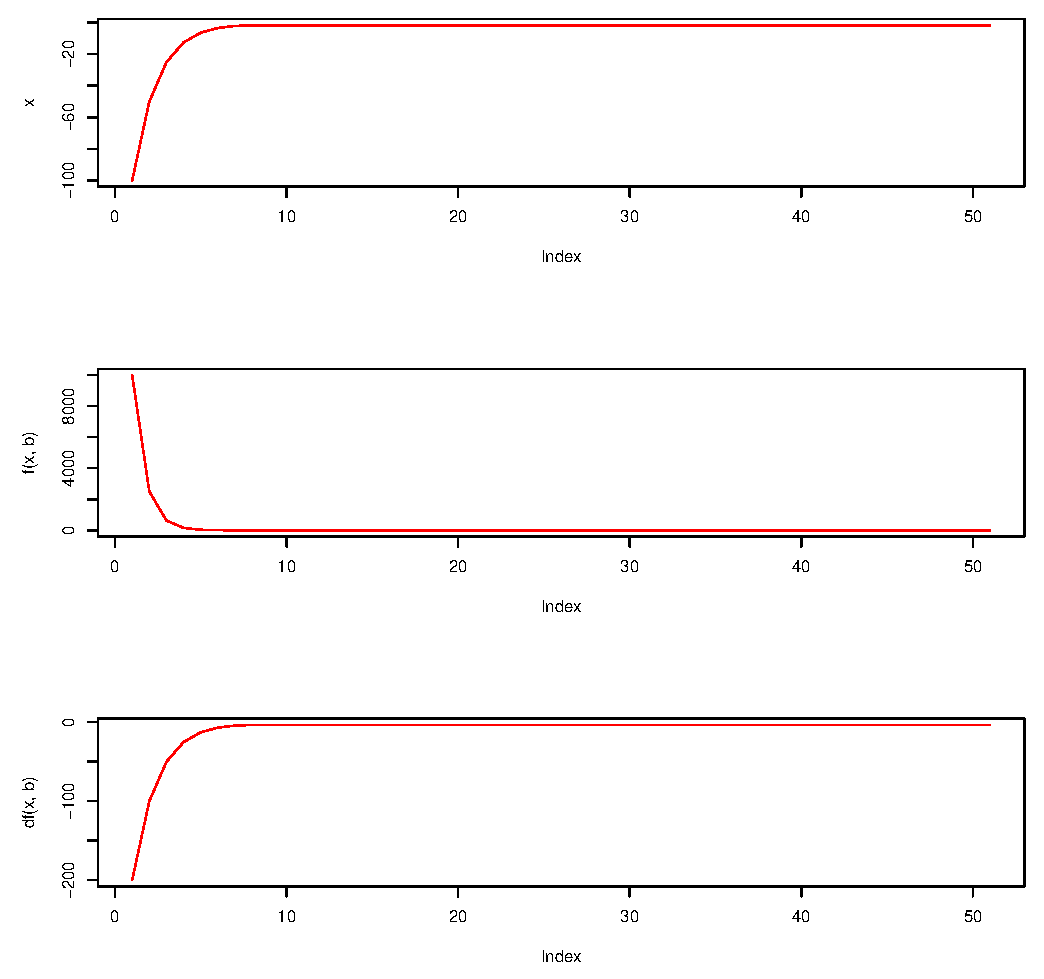
\includegraphics[height=0.92\textheight]{NewtonRaphson}
\end{figure}
\end{frame}

\begin{frame}
  \frametitle{Find the Maximum via Newton-Raphson Algorithm}

  \begin{itemize}

  \item Find $max~ f(x)$ can be viewed as to find the root of

      \begin{align*}
      \frac{\partial f(x)}{\partial x} & =0\\
      \end{align*}

    \item The algorithm is now as

      \begin{align*}
        x_{n+1} = x_n - \left( \frac{\partial ^2 f(x)}{\partial x^2}
           \right)^{-1} \frac{\partial f(x)}{\partial x} \mid_{x=x_n}
      \end{align*}

    \item The second order partial derivative is known as \textbf{Hessian}

  \item The Newton-Raphson algorithm cannot always find the maximum of
    $h(x)$, but rather converges to whatever mode is closest to the
      starting point.
  \end{itemize}
\end{frame}



\begin{frame}
  \frametitle{Example}

  \begin{itemize}
  \item Assume we want to find the maximum value of of $ax^2+bx+c$ by using
    numerical method ($a<0$).

  \item First we have
    \begin{align*}
      f'(x) = 2ax + b\\
      f''(x) = 2a
    \end{align*}

  \item Then

    \begin{equation*}
        x_{n+1} = x_n - \left( 2a \right)^{-1} (2ax_n+b)
    \end{equation*}

  \end{itemize}

\end{frame}


\begin{frame}[fragile]
\begin{verbatim}
## The target function
f <- function(x, a, b, c) a*x^2 +b*x +c
## The gradient wrt x
df <- function(x, a, b, c) 2*a*x +b
## The Hessian wrt x
d2f <- function(x, a, b, c) 2*a
## Loop to find the best x
n <- 50
x <- rep(NA, 1)
a <- -1
b <- 3
c <- 10
x[1] <- -100 # The initial value
for(i in 1:n)
{
    x[i+1] <- x[i]- (d2f(x[i], a, b, c))^(-1)*df(x[i], a, b, c)
}
\end{verbatim}
\end{frame}

\begin{frame}
\frametitle{Diagnosis}

\begin{figure}
  \centering
  \includegraphics[width=\textwidth]{NewtonRaphsonMax}
\end{figure}
\end{frame}

\section{Newton-Raphson Algorithm: The Matrix Version}
\begin{frame}
  \frametitle{Newton-Raphson Algorithm: The Matrix Version}
  \begin{itemize}
  \item The Newton-Raphson algorithm for finding the maximum value of
    $f(\bm{x})$ where $x$ now is a $p\times 1$ vector can be naturally extended as
    \begin{align*}
      \bm{x}_{n+1} = \bm{x}_n - \left( \frac{\partial ^2
          f(\bm{x})}{\partial \bm{x} \partial \bm{x}'}
      \right)^{-1} \frac{\partial f(\bm{x})}{\partial \bm{x}} \mid_{\bm{x}=\bm{x}_n}
    \end{align*}

  \item Note the dimensions of each elements.

  \end{itemize}
\end{frame}

\begin{frame}[allowframebreaks]
\frametitle{Preliminaries for matrix derivatives}

\begin{enumerate}
\item The derivative of a vector $\mathbf{y} = \begin{bmatrix} y_1 \\ y_2 \\ \vdots \\ y_m \\ \end{bmatrix}$ , by a scalar $x$ is written (in numerator layout notation) as
  \begin{align*}
    \frac{\partial \mathbf{y}}{\partial x} = \begin{bmatrix} \frac{\partial y_1}{\partial x}\\ \frac{\partial y_2}{\partial x}\\ \vdots\\ \frac{\partial y_m}{\partial x}\\ \end{bmatrix}.
  \end{align*}
In vector calculus the derivative of a vector $y$ with respect to a scalar $x$ is known as the tangent vector of the vector $y$, $\frac{\partial \mathbf{y}}{\partial x}$

\item \textbf{The derivative of a scalar $y$ by a vector} $\mathbf{x} = \begin{bmatrix} x_1 \\ x_2 \\ \vdots \\ x_n \\ \end{bmatrix}$ , is written (in numerator layout notation) as
  \begin{align*}
    \frac{\partial y}{\partial \mathbf{x}} = \left[ \frac{\partial y}{\partial x_1} \ \ \frac{\partial y}{\partial x_2} \ \ \cdots \ \ \frac{\partial y}{\partial x_n} \right].
  \end{align*}

\item \textbf{The second order derivatives of a scalar $y$ by a vector} $\mathbf{x}
  = \begin{bmatrix} x_1 \\ x_2 \\ \vdots \\ x_n \\ \end{bmatrix}$ is written (in numerator layout notation) as

  \begin{align*}
    \frac{\partial^2 y}{\partial \mathbf{x}\partial \mathbf{x}'}&=\frac{\partial
    }{\partial \mathbf{x}'}\left[\frac{\partial y}{\partial \mathbf{x}}\right]=\frac{\partial}{\partial \mathbf{x}'}\left[ \frac{\partial y}{\partial x_1} \ \ \frac{\partial y}{\partial x_2} \ \ \cdots \ \ \frac{\partial y}{\partial x_n} \right] \\&= \begin{bmatrix} \frac{\partial^2 y}{\partial x_1^2} & \frac{\partial^2 y}{\partial x_1\partial x_2} & \cdots & \frac{\partial^2 y}{\partial x_1\partial x_n}\\ \frac{\partial^2 y}{\partial x_2\partial x_1} & \frac{\partial^2 y}{\partial x_2^2} & \cdots & \frac{\partial^2 y}{\partial x_2\partial x_n}\\ \vdots & \vdots & \ddots & \vdots\\ \frac{\partial^2 y}{\partial x_m\partial x_1} & \frac{\partial^2 y}{\partial x_m\partial x_2} & \cdots & \frac{\partial^2 y}{\partial x_m\partial x_m}\\ \end{bmatrix}.
  \end{align*}

\item The derivative of a vector function (a vector whose components are functions) $\mathbf{y} = \begin{bmatrix} y_1 \\ y_2 \\ \vdots \\ y_m \\ \end{bmatrix}$ , with respect to an input vector, $\mathbf{x} = \begin{bmatrix} x_1 \\ x_2 \\ \vdots \\ x_n \\ \end{bmatrix}$ , is written (in numerator layout notation) as

  \begin{align*}
    \frac{\partial \mathbf{y}}{\partial \mathbf{x}} = \begin{bmatrix} \frac{\partial y_1}{\partial x_1} & \frac{\partial y_1}{\partial x_2} & \cdots & \frac{\partial y_1}{\partial x_n}\\ \frac{\partial y_2}{\partial x_1} & \frac{\partial y_2}{\partial x_2} & \cdots & \frac{\partial y_2}{\partial x_n}\\ \vdots & \vdots & \ddots & \vdots\\ \frac{\partial y_m}{\partial x_1} & \frac{\partial y_m}{\partial x_2} & \cdots & \frac{\partial y_m}{\partial x_n}\\ \end{bmatrix}.
  \end{align*}

\item The derivative of a matrix function $Y$ by a scalar $x$ is known as the tangent
  matrix and is given (in numerator layout notation) by
  \begin{align*}
    \frac{\partial \mathbf{Y}}{\partial x} = \begin{bmatrix} \frac{\partial y_{11}}{\partial x} & \frac{\partial y_{12}}{\partial x} & \cdots & \frac{\partial y_{1n}}{\partial x}\\ \frac{\partial y_{21}}{\partial x} & \frac{\partial y_{22}}{\partial x} & \cdots & \frac{\partial y_{2n}}{\partial x}\\ \vdots & \vdots & \ddots & \vdots\\ \frac{\partial y_{m1}}{\partial x} & \frac{\partial y_{m2}}{\partial x} & \cdots & \frac{\partial y_{mn}}{\partial x}\\ \end{bmatrix}.
  \end{align*}

\item The derivative of a scalar $y$ function of a matrix $X$ of independent variables, with respect to the matrix $X$, is given (in numerator layout notation) by

  \begin{align*}
    \frac{\partial y}{\partial \mathbf{X}} = \begin{bmatrix} \frac{\partial y}{\partial x_{11}} & \frac{\partial y}{\partial x_{21}} & \cdots & \frac{\partial y}{\partial x_{p1}}\\ \frac{\partial y}{\partial x_{12}} & \frac{\partial y}{\partial x_{22}} & \cdots & \frac{\partial y}{\partial x_{p2}}\\ \vdots & \vdots & \ddots & \vdots\\ \frac{\partial y}{\partial x_{1q}} & \frac{\partial y}{\partial x_{2q}} & \cdots & \frac{\partial y}{\partial x_{pq}}\\ \end{bmatrix}.
  \end{align*}

\end{enumerate}

%\includegraphics[width=\textwidth]{Matrix-Derivatives.pdf}

\end{frame}

\begin{frame}
\frametitle{The linear regression model, a revisit}
\begin{itemize}
\item Consider the linear regression model with multiple covariates,

  \begin{equation*}
    y_i = \beta_0 + \beta_1x_1+...+\beta_p x_p + \epsilon_i
  \end{equation*}
where $\epsilon_i \sim N(0, \sigma^2)$

\item What is the gradient and Hessian matrix for the log likelihood ($\mathcal{L}$)
  with respect to the parameter vector $\bm{\beta}=(\beta_0,...,\beta_p)$?

  \begin{equation*}
    \frac{\partial log \mathcal{L}}{\partial \bm{\beta}} = ?
  \end{equation*}

  \begin{equation*}
    \frac{\partial^2 log \mathcal{L}}{\partial \bm{\beta} \partial \bm{\beta}'}
    = ?
  \end{equation*}

\end{itemize}
\end{frame}

\begin{frame}
  \frametitle{Vector Newton-Raphson Algorithm: The logit model}
  \framesubtitle{Estimate logit model with ungrouped (individual) data}
  \begin{itemize}
  \item \textbf{The idea}: using maximum likelihood method with binomial
    distribution.
  \item One owns a house ($Y=1$) or do not own a house ($Y=0$) can be
    represented with \textbf{Bernoulli distribution}
    \begin{equation*}
      Pr(y;p) = p^y (1-p)^{1-y}\!\quad \text{for }y\in\{0,1\}.
    \end{equation*}
  \item The log likelihood function is as follows
    \begin{equation*}
      \begin{split}
        l(\beta)=& \sum \limits_{n=1}^N\left\{ y_i \log P_i + (1- y_i)
          \log (1-P_i)  \right\}\\
        % =& \sum \limits_{n=1}^N \left\{y_i\beta'x_i -(1-y_i)\log (1+\exp\{1+\beta'x_i\})  \right\}
      \end{split}
    \end{equation*}
    where
    \begin{equation*}
      P_i=\frac{1}{1+\exp(-(\beta_1+\beta_2X_{2i}+...+\beta_pX_{pi}))}
    \end{equation*}

  \item Note that the sum of $n$ Bernoulli samples will be \textbf{binomial}
    distributed.

  \item To obtain $\hat \beta$, use Newton-Raphson algorithm
    \begin{equation*}
      \beta^{new} = \beta^{old} - \left(\frac{\partial^2l(\beta)}{\partial
          \beta\partial \beta'}  \right)^{-1} \frac{\partial
        l(\beta)}{\partial\beta} | _{\beta= \beta^{old}}
    \end{equation*}

  \end{itemize}
\end{frame}


\section{Proof of quadratic convergence for Newton's method}

\begin{frame}[allowframebreaks]

\frametitle{Proof of quadratic convergence for Newton's method}

According to Taylor's theorem, any function $f(x)$ which has a
continuous second derivative can be represented by an expansion about
a point that is close to a root of $f(x)$. Suppose this root is $\alpha
\,$. Then the expansion of $f(\alpha)$ about $x_n$ is:

\begin{equation*}
    f(\alpha) = f(x_n) + f^\prime(x_n)(\alpha - x_n) + R_1 \,
  \end{equation*}

where the Lagrange form of the Taylor series expansion remainder is

\begin{equation*}
    R_1 = \frac{1}{2!}f^{\prime\prime}(\xi_n)(\alpha - x_n)^{2} \,,
  \end{equation*}

where $xi_n$ is in between $x_n$ and $\alpha \,$.

Since $\alpha \,$ is the root, (1) becomes:

\begin{equation*}
    0 = f(\alpha) = f(x_n) + f^\prime(x_n)(\alpha - x_n) + \frac{1}{2}f^{\prime\prime}(\xi_n)(\alpha - x_n)^{2} \,
  \end{equation*}

Dividing equation (2) by $f^\prime(x_n)\,$ and rearranging gives

\begin{equation*}
    \frac {f(x_n)}{f^\prime(x_n)}+\left(\alpha-x_n\right) = \frac {- f^{\prime\prime} (\xi_n)}{2 f^\prime(x_n)}\left(\alpha-x_n\right)^2
  \end{equation*}

Remembering that $x_{n+1}$ is defined by

\begin{equation*}
  x_{n+1} = x_{n} - \frac {f(x_n)}{f^\prime(x_n)} \,
\end{equation*}

one finds that

\begin{equation*}
    \underbrace{\alpha - x_{n+1}}_{\epsilon_{n+1}} = \frac {- f^{\prime\prime} (\xi_n)}{2 f^\prime(x_n)} (\underbrace{\alpha - x_n}_{\epsilon_{n}})^2 \,.
  \end{equation*}
That is,

\begin{equation*}
    \epsilon_{n+1} = \frac {- f^{\prime\prime} (\xi_n)}{2 f^\prime(x_n)} \, {\epsilon_n}^2 \,.
  \end{equation*}

Taking absolute value of both sides gives

\begin{equation*}
    \left| {\epsilon_{n+1}}\right| = \frac {\left| f^{\prime\prime} (\xi_n) \right| }{2 \left| f^\prime(x_n) \right|} \, {\epsilon_n}^2 \,
  \end{equation*}


The equation shows that the rate of convergence is quadratic if
following conditions are satisfied:


$f'(x)\ne0; \forall x\in I \text{, where }I \text{ is the interval
}[\alpha-r,\alpha+r]\text{ for some } r \ge
\left\vert(\alpha-x_0)\right\vert;\, f''(x) \text{ is finite },\forall
x\in I; \, x_0 \, \text{sufficiently close to the root}~ \alpha \,$


The term sufficiently close in this context means the following:

(a) Taylor approximation is accurate enough such that we can ignore higher order terms,

(b)
\begin{equation*}
\frac 1 {2}\left |{\frac {f^{\prime\prime} (x_n)}{f^\prime(x_n)}}\right |<C\left |{\frac {f^{\prime\prime} (\alpha)}{f^\prime(\alpha)}}\right |, \text{ for some } C<\infty,\,
\end{equation*}


(c)
\begin{equation*}
C \left |{\frac {f^{\prime\prime} (\alpha)}{f^\prime(\alpha)}}\right
|\epsilon_n<1, \text{ for }n\in Z^+ \cup \{0\} \text{ and }C \text{ satisfying condition (b) }.\,
\end{equation*}

Finally, it can be expressed in the following way:

\begin{equation*}
    \left | {\epsilon_{n+1}}\right | \le M{{\epsilon}^2}_n \,
  \end{equation*}
where M is the supremum of the variable coefficient of ${\epsilon^2}_n \,$ on the interval I\, defined in the condition 1, that is:

\begin{equation*}
M = \sup_{x \in I} \frac 1 {2}\left |{\frac {f^{\prime\prime} (x)}{f^\prime(x)}}\right |. \,
\end{equation*}
The initial point $x_0 \,$ has to be chosen such that conditions 1 through 3 are satisfied, where the third condition requires that $M\left |\epsilon_0 \right |<1.\,$
\end{frame}

\section{Optimizing the likelihood function}


\begin{frame}
  \frametitle{Maximum likelihood Estimate for linear models}

  \begin{itemize}
  \item Assume you want to make a regression model

    \begin{equation*}
      y_i = \beta_0 + \beta_1 x_i + \epsilon_i
    \end{equation*}

    where $\epsilon_i \sim N(0, \sigma^2)$

  \item What is the (log) likelihood function?

  \item What are the unknown parameters?

  \item How do we estimate the parameters? Let's consider three situations


    \begin{itemize}
    \item When $\beta_0=1$ and $\sigma^2=1$ known.
    \item When $\sigma^2=1$ known.
    \item Neither $\beta$ nor $\sigma$ is known.
    \end{itemize}

    \item Write down the likelihood function with respect to the
      unknown parameters.

    \item Write down the gradient for the likelihood function.

    \item Write down the Hessian for the likelihood function.

    \item Use Newton's method to obtain the best parameter estimate.

  \end{itemize}

\end{frame}

\begin{frame}[fragile]
  \frametitle{Optimizing the likelihood function by using \texttt{optim()}}



\begin{verbatim}
## Generate some data
beta0 <- 1
beta1 <- 3
sigma <- 1
n <- 1000
x <- rnorm(n, 3, 1)
y <- beta0 +x*beta1 + rnorm(n, mean = 0, sd = sigma)
plot(x, y, col = "blue", pch = 20)

## The optimization
optimOut <- optim(c(0, -1, 0.1), logNormLikelihood,
                  control = list(fnscale = -1),
                  x = x, y = y)
beta0Hat <- optimOut$par[1]
beta1Hat <- optimOut$par[2]
sigmaHat <- optimOut$par[3]
yHat <- beta0Hat + beta1Hat*x

plot(x, y, pch = 20, col = "blue")
points(sort(x), yHat[order(x)], type = "l", col = "red", lwd = 2)
\end{verbatim}
\end{frame}


\begin{frame}[fragile]
\frametitle{Comparison with OLS}

\begin{verbatim}
myLM <- lm(y~x)
myLMCoef <- myLM$coefficients
yHatOLS <- myLMCoef[1] + myLMCoef[2]*x

plot(x, y, pch = 20, col = "blue")
points(sort(x), yHat[order(x)], type = "l", col = "red", lwd = 10)
points(sort(x), yHatOLS[order(x)], type = "l",
       col = "blue", lty="dashed", lwd = 2, pch = 20)
\end{verbatim}
\end{frame}


\begin{frame}[plain]
  \begin{figure}
    \centering
    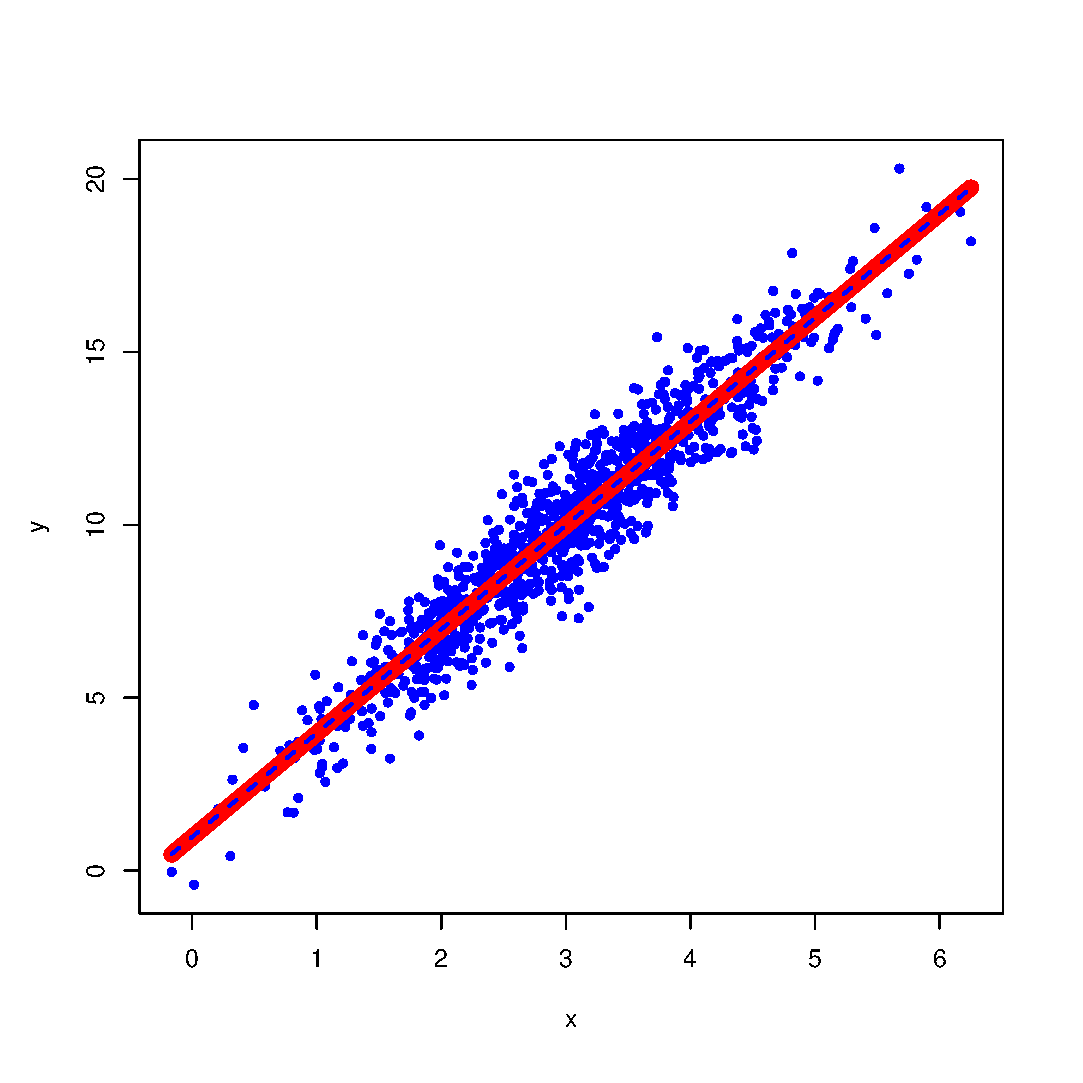
\includegraphics[height=\textheight]{OLSvsML}
  \end{figure}
\end{frame}

\begin{frame}
  \frametitle{Discussions}

  \begin{itemize}
  \item How does the initial values help the optimization algorithm?
    Try with a few different numbers.

  \item Is there anything can be improved in the likelihood function?

  \item The importance of independence.
  \end{itemize}
\end{frame}

\begin{frame}
  \frametitle{Lab exercise}

  % Submit your R code of this lab exercises online to the course
  % page. The due date is \textbf{April 8 @ 24hrs}.

    \begin{enumerate}
    \item Generate 1000 random numbers $\epsilon_i$ from student t distribution
      with 3 degrees of freedom [\texttt{rt()}]. Generate a covariate $x$
      from $N(1,1)$. Let $\beta_0=1,\beta_1=-1$. Now generate $y$ with
      the model

      \begin{equation*}
        y_i= \beta_0 + \beta_1 x_i + \epsilon_i
      \end{equation*}

    \item Use OLS method to estimate a linear model given $y$ and $x$
      [\texttt{lm()}].

    \item Estimate the model with the maximum likelihood method.

    \item Compare the two results with a plot.
    \end{enumerate}
  \end{frame}


\section{The steepest ascent algorithm}

\begin{frame}[allowframebreaks]
  \frametitle{The steepest ascent algorithm}

  \begin{itemize}
  \item Let $f(x)$ be a function with continuous partial derivatives everywhere.  We wish
    to find a local maximum of $f(x)$ in the vicinity of some point $x(0)$.

  \item In the \textbf{steepest ascent method}, we put

    \begin{align*}
x(n + 1) = x(n) + \alpha f'(x)
    \end{align*}

    where $\alpha\geq 0$ is a positive scalar and the direction $v$ is the direction with
    largest slope.


  \item To complete the steepest ascent algorithm, at each step $n$ we need to maximize

    \begin{align*}
      g(\alpha) = f(x(n) + \alpha + f'(x))
    \end{align*}

  \newpage
  \item As finding a global maximum of $g(\alpha)$ is hard, we will instead look for a
    local maximum, for which we will use the \textbf{golden-section algorithm}.

    \begin{enumerate}
    \item Let $[a, b]$ be interval of current bracket. $g(a)$, $g(b)$ would already have
      been computed earlier. Let $\phi = (\sqrt{5}-1)/2$

    \item Let $c = b + \phi (a - b)$, $d = a + \phi (b - a)$. If $g(c)$, $g(d)$ not available,
      compute them.

    \item If $g(c) > g(d)$ (this is to find max, to find min, just reverse it) then move
      the data: $(b, g(b)) \leftarrow (d, g(d))$, $(d, g(d)) \leftarrow (c, g(c))$ and
      update $c = b + \phi (a - b)$ and $g(c)$;

    \item Otherwise, move the data: $(a, f(a)) \leftarrow (c, f(c))$,
      $(c, f(c)) \leftarrow (d, f(d))$ and update $d = a + \phi (b - a)$ and $f(d)$.

    \item At the end of the iteration, $[a, c, d, b]$ bracket the maximum point.

    \end{enumerate}


  \end{itemize}

\end{frame}


\section{Diagnosing Convergence}
\begin{frame}
  \frametitle{Diagnosing Convergence}

  \begin{itemize}
  \item We need a \textbf{stopping rule} to guarantee that the number of
    iterations is sufficient.

  \item Criteria

    \begin{itemize}
    \item Convergence to the Stationary Distribution
    \item Convergence of Averages
    \item Convergence to iid Sampling
    \end{itemize}
  \end{itemize}

\end{frame}


\begin{frame}
  \frametitle{Convergence in multiple chains}

  \begin{itemize}
  \item Many multiple-chain convergence diagnostics are quite elaborate.
  \item The performances of these parallel methods require a degree of a priori
    knowledge on the distribution in order to construct an initial
    distribution.


    \begin{itemize}
    \item An initial distribution which is too concentrated around a local mode
      does not contribute significantly more than a single chain to the
      exploration

    \item Moreover, slow algorithms, Gibbs sampling used in highly nonlinear
      setups, usually favor single chains.

    \end{itemize}


  \item It is somewhat of an illusion to think we can control the flow of a
    Markov chain and assess its convergence behavior from a few realizations of
    this chain.

  \end{itemize}
\end{frame}

\begin{frame}
  \frametitle{Monitoring Convergence of Distribution}

  \begin{itemize}
  \item A natural empirical approach to convergence control is to draw pictures
    of the output of simulated chains, in order to detect deviant or
    non-stationary behaviors. However, this plot is only useful for strong
    non-stationarities of the chain.

  \item Tests for non-stationary checking.

    \begin{itemize}
    \item Autocorrelation functions.
    \end{itemize}

  \item Another approach to convergence monitoring is to assess how much of the
    support of the target distribution has been explored by the chain via an
    evaluation of
    \begin{equation*}
      \int_A f(x) dx \approx \sum_{t=1}^{T-1}(\theta(t+1)-\theta_t) f(\theta_t)
    \end{equation*}
    when $f(x)$ is a one-dimensional density, the above converges to 1.

  \end{itemize}

\end{frame}


\begin{frame}
  \frametitle{Monitoring Convergence of Average}

  \begin{itemize}
  \item Graphical outputs can detect obvious problems of convergence of the
    empirical average.

  \item One may use cumulative sums (CUSUM), graphing the partial differences
    \begin{equation*}
      D_T^* \sum _{t=1}^i (h(\theta_t)-\frac{1}{T}\sum_{t=1}^Th(\theta_t))
    \end{equation*}

  \end{itemize}

\end{frame}


\begin{frame}
  \frametitle{Effective Sample Size}
  \begin{itemize}
  \item The standard approach to restore to the \textbf{effective sample size}
    which gives the size of an iid sample with the same variance as the current
    sample and thus indicates the loss in efficiency due to the use of a Markov
    chain. This value is computed as
    \begin{equation*}
      \frac{T}{1+ 2 \sum _{t=1}^{\infty} Corr(h(\theta_0),h(\theta_t))}
    \end{equation*}
    where the denominator is the measurement of efficiency
    (\textbf{inefficiency factor})

  \end{itemize}

\end{frame}

%\section{Sampling techniques}

\begin{frame}
  \frametitle{Suggested Reading}

  \begin{itemize}
  \item Jones (2009), \textbf{Chapter 10, Chapter 12}


  % \emph{Monte Carlo Statistical Methods} Book by Christian P Robert and George
  % Casella. (2004 edition)

  \end{itemize}

\end{frame}

\end{document}
